
\section{React}
\setauthor{David Altenhofer}
React ist eine \textbf{JavaScript-Programmbibliothek} zur Erstellung von webbasierten Benutzeroberflächen. 
Jede React-Webanwendung besteht aus wiederverwendbaren Komponenten, die Teile der Benutzeroberfläche bilden – wir können 
eine separate Komponente für unsere Navigationsleiste haben, eine für die Fußzeile, eine andere für den Hauptinhalt und so weiter. 

Diese wiederverwendbaren Komponenten machen die Entwicklung einfacher, weil man wiederkehrenden Code nicht wiederholen muss. 
Man muss nur die Logik erstellen und die Komponente in jeden Teil des Codes importieren, in dem sie benötigt wird.
React ist außerdem eine Single-Page-Anwendung. Anstatt also jedes Mal, wenn eine neue Seite gerendert werden soll, eine Anfrage 
an den Server zu senden, wird der Inhalt der Seite direkt von den React-Komponenten geladen. Das führt zu einem schnelleren 
Rendering ohne Neuladen der Seite.

In den meisten Fällen wird für die Erstellung von React-Apps die Syntax JSX (JavaScript XML) verwendet, eine Syntaxerweiterung 
von JavaScript. Damit kann man die Logik von JavaScript und die Logik der Benutzeroberfläche auf einzigartige Weise kombinieren. 
Mit JSX muss kein DOM integriert werden, weil man einfach Methoden wie \textbf{document.getElementById}, \textbf{querySelector} 
und andere DOM-Manipulationsmethoden verwendet.
Die Verwendung von JSX ist zwar nicht obligatorisch, aber sie macht die Entwicklung von React-Anwendungen einfacher.


\begin{figure}[ht!]
    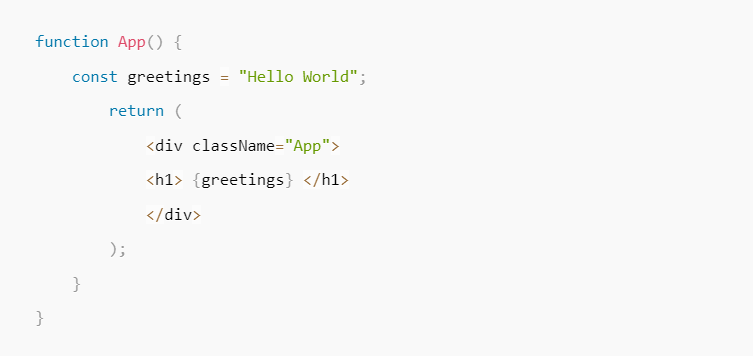
\includegraphics[width=.94\textwidth]{pics/jsx-example.PNG}
    \caption{\label{fig:The-caption}JSX-Example in React \cite{APCW2006}}
  \end{figure}

Im oberen Code-Beispiel wird eine funktionale React-Komponente verwendet, um ein Stück Text im Browser darzustellen. 
Der Name der Komponente ist \textbf{App}. Es wird eine Variable vor der Funktion \textbf{render()} erstellt.
Diese Variable wird mit geschweiften Klammern an das Markup übergeben. Das ist kein HTML, sondern die 
Syntax für das Schreiben von Code mit JSX.

\clearpage

\section{Tailwind CSS}
\setauthor{David Altenhofer}
Tailwind CSS ist ein Utility-First-CSS-Framework. Es stellt vorgefertigte CSS-Klassen bereit, die verwendet 
werden können, um HTML-Elemente schnell und einfach zu gestalten. Im Vergleich mit anderen CSS-Frameworks, 
die vorgefertigte UI-Komponenten bereitstellen, fokussiert sich Tailwind mehr auf Low-Level-Bausteine wie 
Abstände (Paddings und Margins), Schriftarten und Farbe, um benutzerdefinierte Styles zu erstellen.

Entwickler können vorgefertigte CSS-Klassen hinzufügen, anstatt für jedes Element benutzerdefiniertes CSS zu 
schreiben. Das beschleunigt nicht nur den Entwicklungsprozess, sondern kann sich auch positiv auf die Performance 
auswirken. Die Dokumentation von Tailwind CSS ist umfangreich und die große Community erleichtert den Einstieg und 
bietet Unterstützung.

\begin{figure}[ht!]
    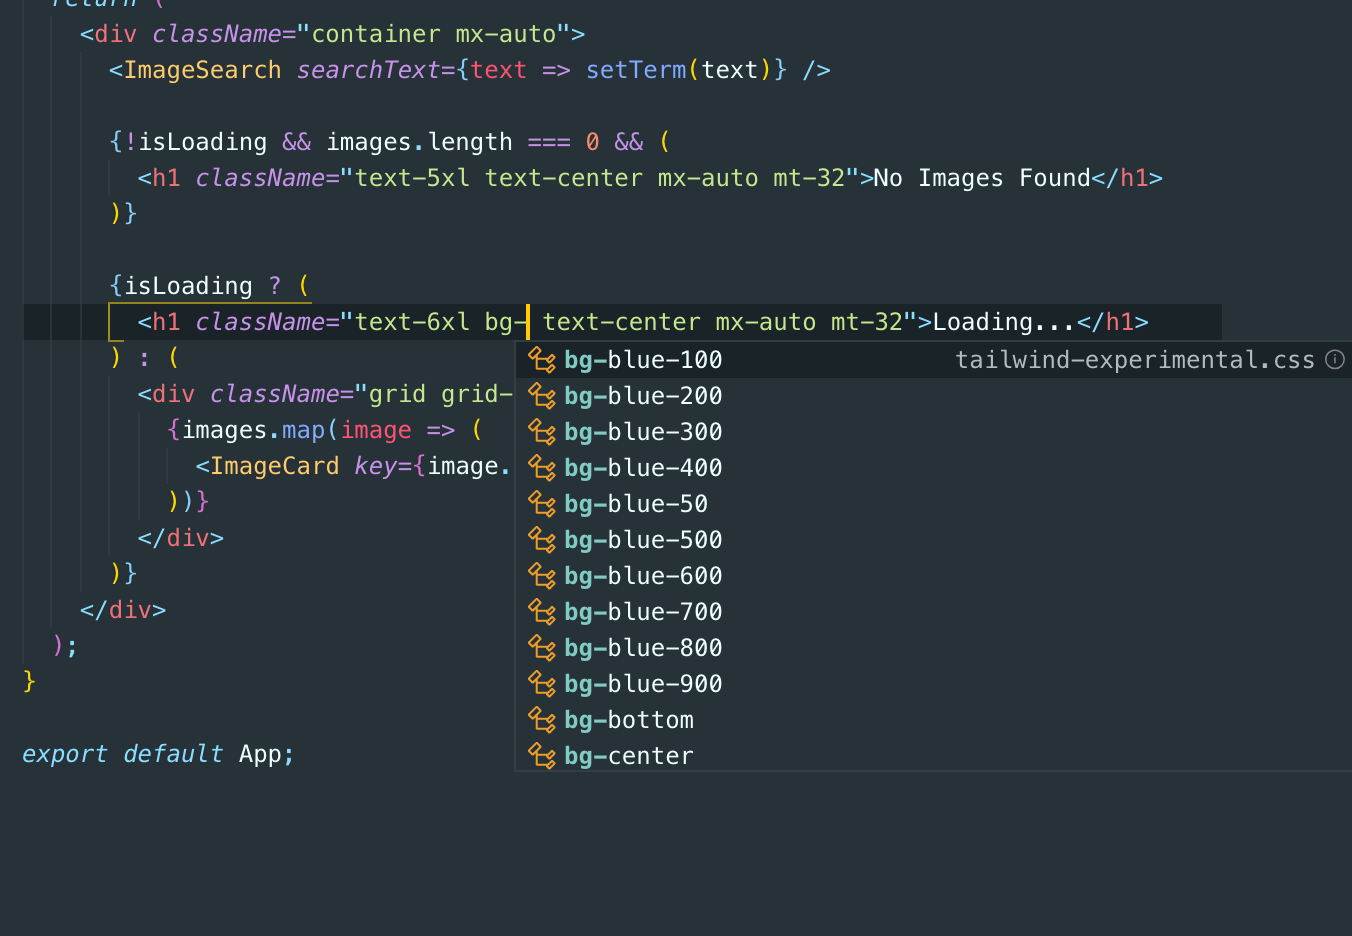
\includegraphics[width=.94\textwidth]{pics/tailwindCSS-class-showcase.png}
    \caption{\label{fig:The-caption}Tailwind - vorgefertigte CSS-Klassen \cite{APCW2006}}
  \end{figure}


\section{Material UI}
\setauthor{David Altenhofer}

\section{Swagger UI}
\setauthor{David Altenhofer}

\section{HTTP-Request / REST}
\setauthor{David Altenhofer}

\section{OAuth}
\setauthor{David Altenhofer}

\section{OIDC}
\setauthor{David Altenhofer}

\section{Dev Ops}
\setauthor{David Altenhofer}


\subsection{Deeper}
Nicht mehr im Inhaltsverzeichnis.
